\subsection{Attention and Transformer} % 2.5 pages
%Attention
\citet{bahdanau2016neural}

\begin{minipage}[]{\textwidth}
\centering
\begin{minipage}[ht]{.52\textwidth}
    \begin{figure}[H]
        \centering
        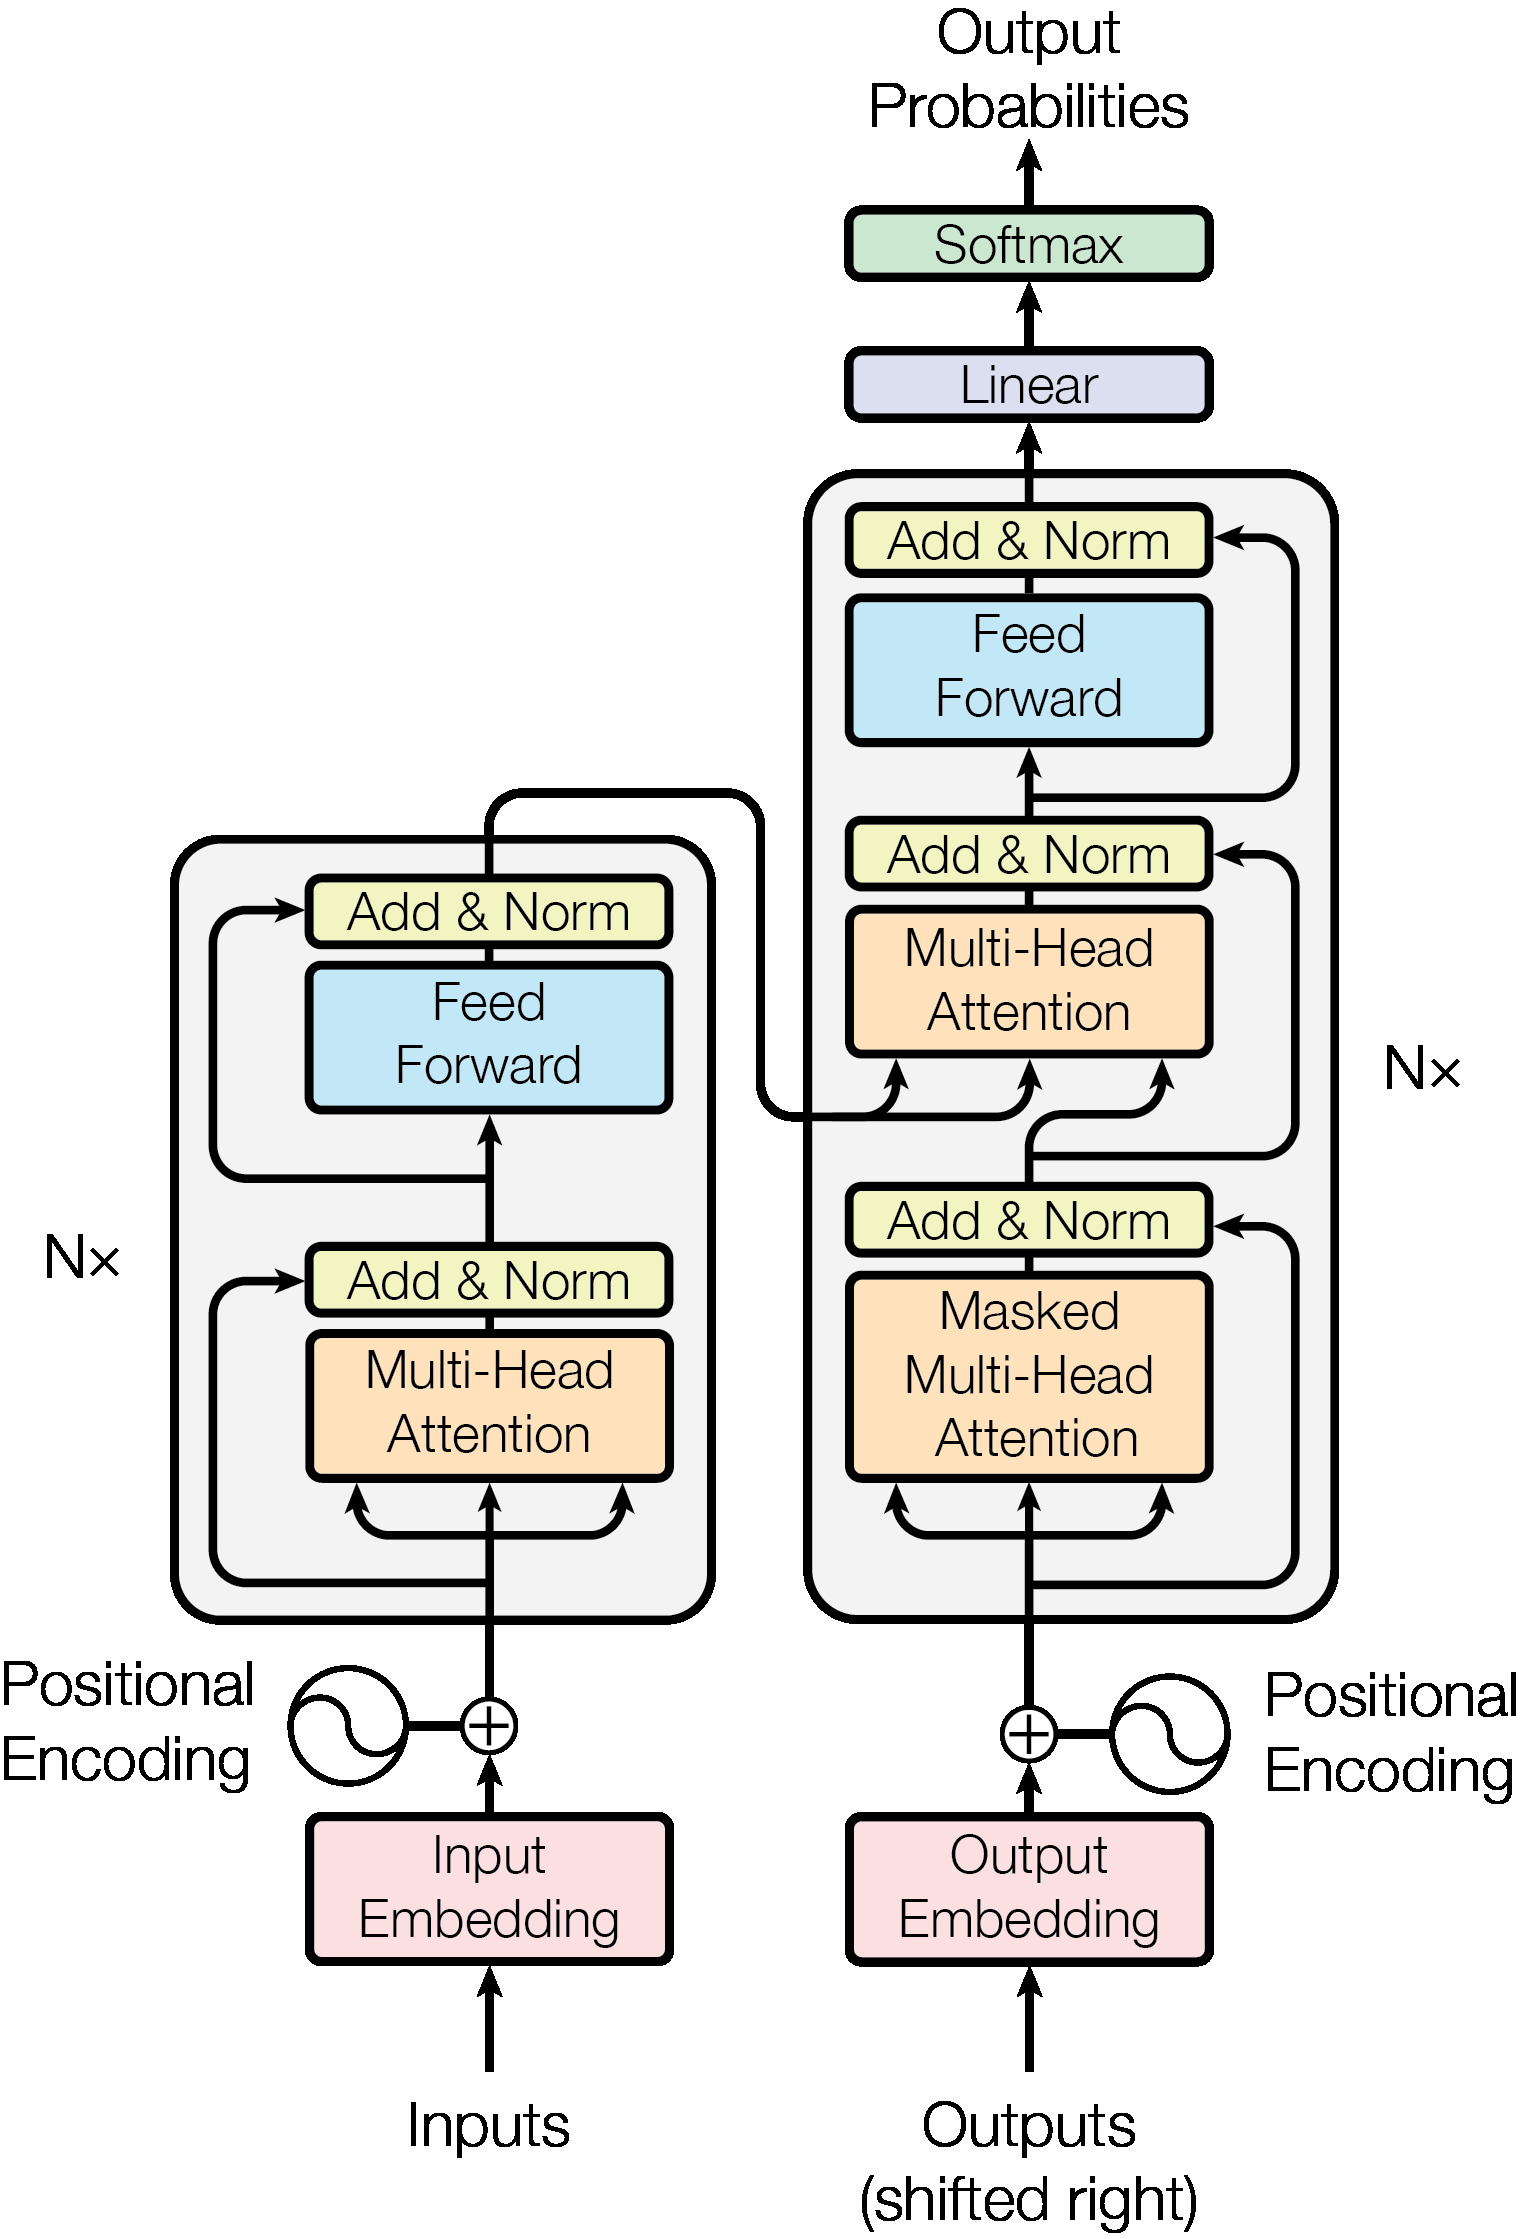
\includegraphics[width=\textwidth]{literature/imgs/ext-transformer.png}
        \caption{The Transformer model architecture \cite{vaswani2017attention}}
        \label{fig:ext-transformer}
    \end{figure}
\end{minipage}
\hspace{1em}
\begin{minipage}[ht]{.35\textwidth}
    \centering
    \begin{figure}[H]
        \centering
        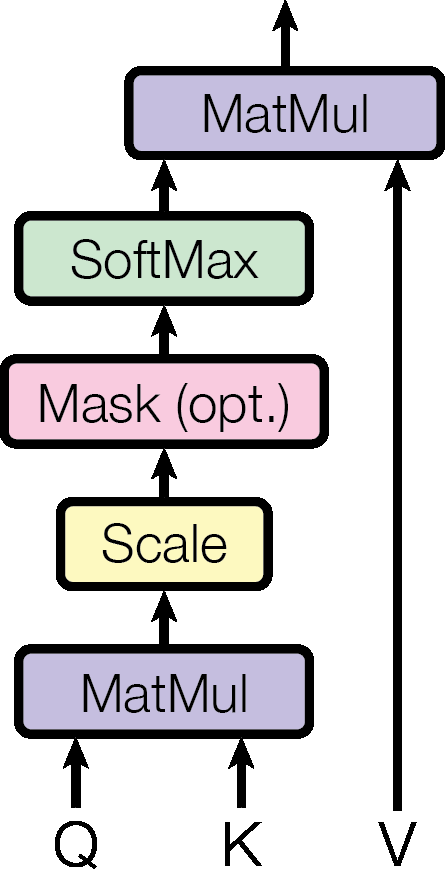
\includegraphics[width=.48\textwidth]{literature/imgs/ext-attention-dot-product.png}
        \caption{Scaled Dot-Product Attention \cite{vaswani2017attention}}
        \label{fig:ext-attention-dot-product}
    \end{figure}
    \vspace*{-.5cm}
    \begin{figure}[H]
        \centering
        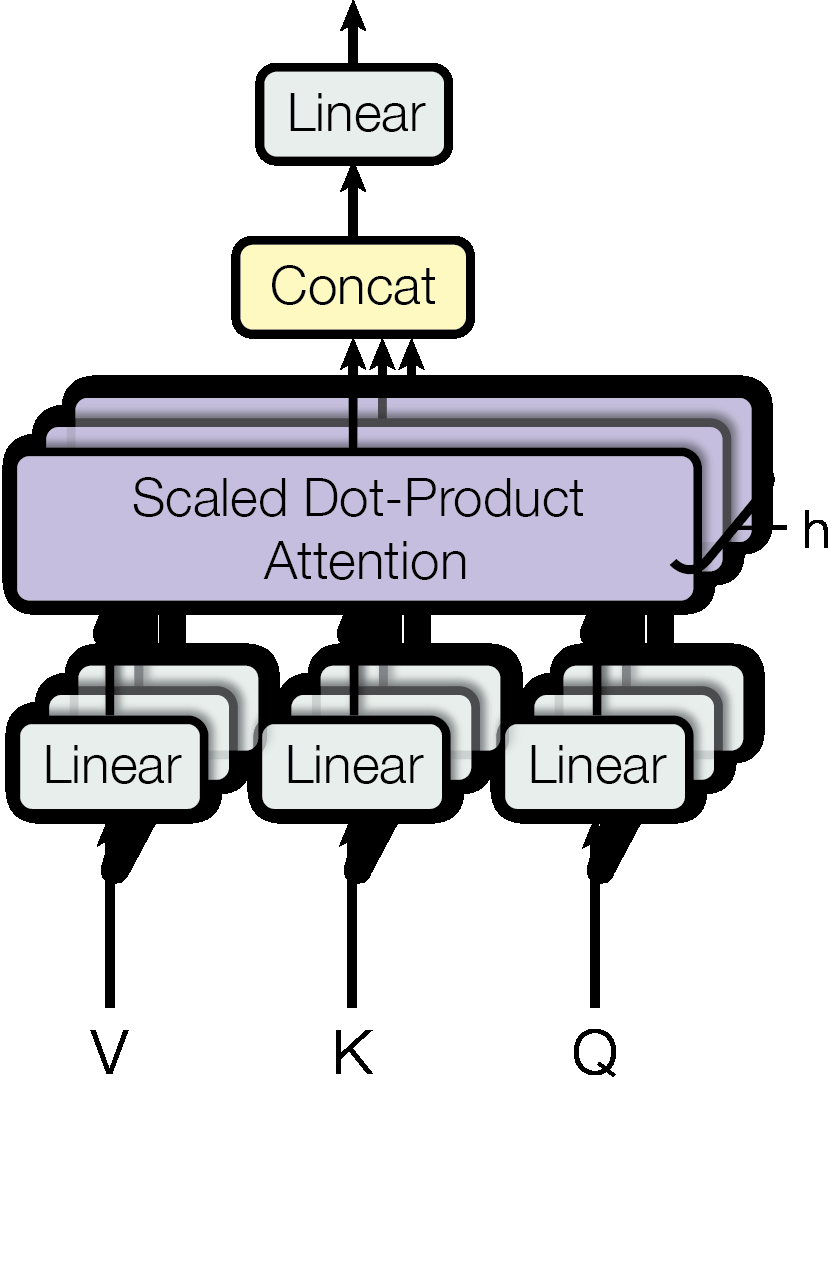
\includegraphics[width=.9\textwidth]{literature/imgs/ext-attention-multihead.png}
        \vspace*{-2em}
        \caption{Multi-Head Attention \cite{vaswani2017attention}}
        \label{fig:ext-attention-multihead}
    \end{figure}
\end{minipage}
\end{minipage}

\citet{vaswani2017attention}

%Transformer
While convolutional neural network (CNN) is in the ascendant among the fields of computer vision, transformer model composed of self-attention structures has achieved state-of-the-art results in many natural language processing tasks.

\citet{devlin2019bert}

The transformer model gradually replaced the recurrent neural network (RRN) with sequential computing restriction and long-term memory loss issues.